\chapter{Fragen zur Vorbereitung}
\section{Aufbau eines Lasers}
Laser sind Strahlungsquellen für 'scharf' gebündelte Strahlung. 
Im Prinzip besteht ein Laser ganz allgemein aus 3 Bestandteilen: 
dem Laseraktiven Medium, der Pumpe und dem Resonator.
\subsection{Lasermedium}
Das Lasermedium ist entscheidend für die Eigenschaften des Lasers, Beispiele 
sind Gase, Kristall oder Dioden.\\
Das Medium muss einige Voraussetzungen erfüllen, es muss sich 
ein sogenannte \textbf{Besetzungsinversion} einstellen können. 
Im thermischen Gleichgewicht ist die Besetzungszahl des Grundzustand 
(bzw. eines niedrigeren energetischen Zustand) meist höher als in 
einem angeregtem Zustand (eines energestisch höheren Zustand). 
Wenn dieser Zustand umgekehrt ist, nennt man das Besetzungsinversion, dies ist 
wichtig um eine Lichtverstärkung zu erreichen.\\
Desweiteren müssen verschieden Vorgänge im Laser passieren, damit dieser funktioniert.
Dazu ist es wichtig zwei Begriffe genauer zu betrachten. 
Bei der \textbf{spontane Emisson} wird ein Photon, aus einem angeregtem Zustand, 
ausgesendet ohne das es zur einer äußeren Einwirkung kommt. Der Übergang von einem angeregtem
Zustand in den Grundzustand (oder einem energestisch niedrigeren Zustand) geschieht hierbei spontan statt, d.h. es ist
ein statistischer Prozess.\\
Wichtig zu klären ist der Begriff der \textbf{induzierte oder stimulierten Emission}.
\subsection{Pumpe}
Mithilfe der Pumpe wird Energie in das Lasermedium zugeführt, z.B. elektrische 
Gasentladungen.
\subsection{Resonator}
Der Laserresonator besteht aus einem Spiegelsystem oder/und anderen optiscshen Elementen.
\section{Besetzungswahrscheinlichkeit, spontane und induzierte Emission, Verstärkung 
eines laseraktiven Mediums}
\section{Homogene und inhomogene Verbreiterung von Spektrallinien, Linienbreite}
\textbf{Homogene und inhomogene Verbreiterung von Spektrallinien:}\\
Ist die Wahrscheinlichtkeit für den Übergang eines Zustandes $E_2$ nach $E_1$ für alle Atome/Moleküle im Zustand $E_2$ gleich, ist das Spektralprofil homogen.
Somit ist die entsprechende Absorptions-/ Emissionslinie homogen verbreitert.\\
Ist die Wahrscheinlichtkeit für den Übergang nicht für alle Atome gleich, ist das Spektralprofil inhomogen.
Somit folgt eine inhomogene Verbreiterung der Spektrallinien.
Dies ist beispielsweise der der Doppler-Verbreiterung der Fall.
Dort hängt die Wahrscheinlichtkeit von der Geschwindigkeit der Moleküle ab.
Diese Bewegen sich auf dem Detektor zu und wieder weg, was eine Änderung der Frequenz zur Folge hat (Doppler-Effekt).\\\\
\textbf{Linienbreite:}\\
Spektrallinien sind im echten Leben, keine $\delta$-Funktionen, sondern haben aufgrund der Quantenmechanischen Unschärfe eine endliche Breite.
Diese Linienbreite bezeichnet die Länge eines Intervalles eines Frequenzspektrums, welches von einer Spektrallinie überdeckt wird.
\section{Optische Resonatoren, Schwingungsmoden, Abstand von Axialmoden, Bandbreite von Laser-Oszillatoren, single-mode Betrieb eines Lasers}
\textbf{Optische Resonatoren:}\\
Optische Resonatoren werden verwendet, um das Laserlicht zu verstärken.
Dies wird dadurch erreicht, das der Resonator für die gewünschten Moden eine strake Rückkopplung hat.
Dies ist erfüllt, wenn der optische Weg im Resonator ein Vielfaches des halben Wellenlänge des Lichtes ist.
In einem Laser wird dies mit einer Anordnung von Spiegeln realisiert.\\\\
\textbf{Schwingungsmoden:}\\
Die Mode beschreibt eine bestimmte zeitliche stationäre Eigenschaft einer Welle (Stehende Welle).
Die Form der Moden wird meist durch Randbedingungen bestimmt.\\
Bei elektro-magnetischen Wellen unterscheidet man folgende Moden-Formen:
\begin{itemize}
    \item \textbf{TEM}:
    Elektrische und magnetische Feldkomponente stehen senkrecht zur Ausbreitungsrichtung.
    \item \textbf{TE}:
    Elektrische Feldkomponente steht senkrecht zur Ausbreitungsrichtung. Die magnetische Feldkomponente zeigt in Ausbreitungsrichtung.
    \item \textbf{TM}:
    Magnetische Feldkomponente steht senkrecht zur Ausbreitungsrichtung. Die elektrische Feldkomponente zeigt in Ausbreitungsrichtung.
\end{itemize}
\textbf{Abstand von Axialmoden:}\\
Bei Axialmoden ist die Ausbreitungsrichtung entlang der optischen Achse des Resonators.
Für den Abstand zweier Axialmoden nehmen wir die Bedingung für ein Verstärkung innerhalb des Resonators her:
\begin{equation}
    L=k\frac{\lambda}{2}
\end{equation}
Hier steht $L$ für die Länge des Resonators, $\lambda$ der Wellenlänge des emittierten Lichts und $k$ für eine natürliche Zahl.
Setzen wir nun für die Wellenlänge $c'=\nu\lambda$, mit $c'$ der Ausbreitungsgeschwindigkeit im Medium $c=c'n$ folgt:
\begin{align}
    L&=k\frac{\lambda}{2}\\
    L&=k\frac{c'}{2\nu}\\
    \nu&=\frac{ck}{2Ln}
\end{align}
Nun Bertrachen wir den Abstand zweier benachbarter:
\begin{align}
    \nu_{k+1}-\nu_k&=\frac{c(k+1)}{2Ln}-\frac{ck}{2Ln}\\
    \nu_{k+1}-\nu_k&=\frac{ck}{2Ln}
\end{align}
\textbf{Bandbreite von Laser-Oszillatoren:}\\
Die Bandbreite eines Lasers sieht wie folgt aus:
\begin{center}
    \begin{figure}[h]
        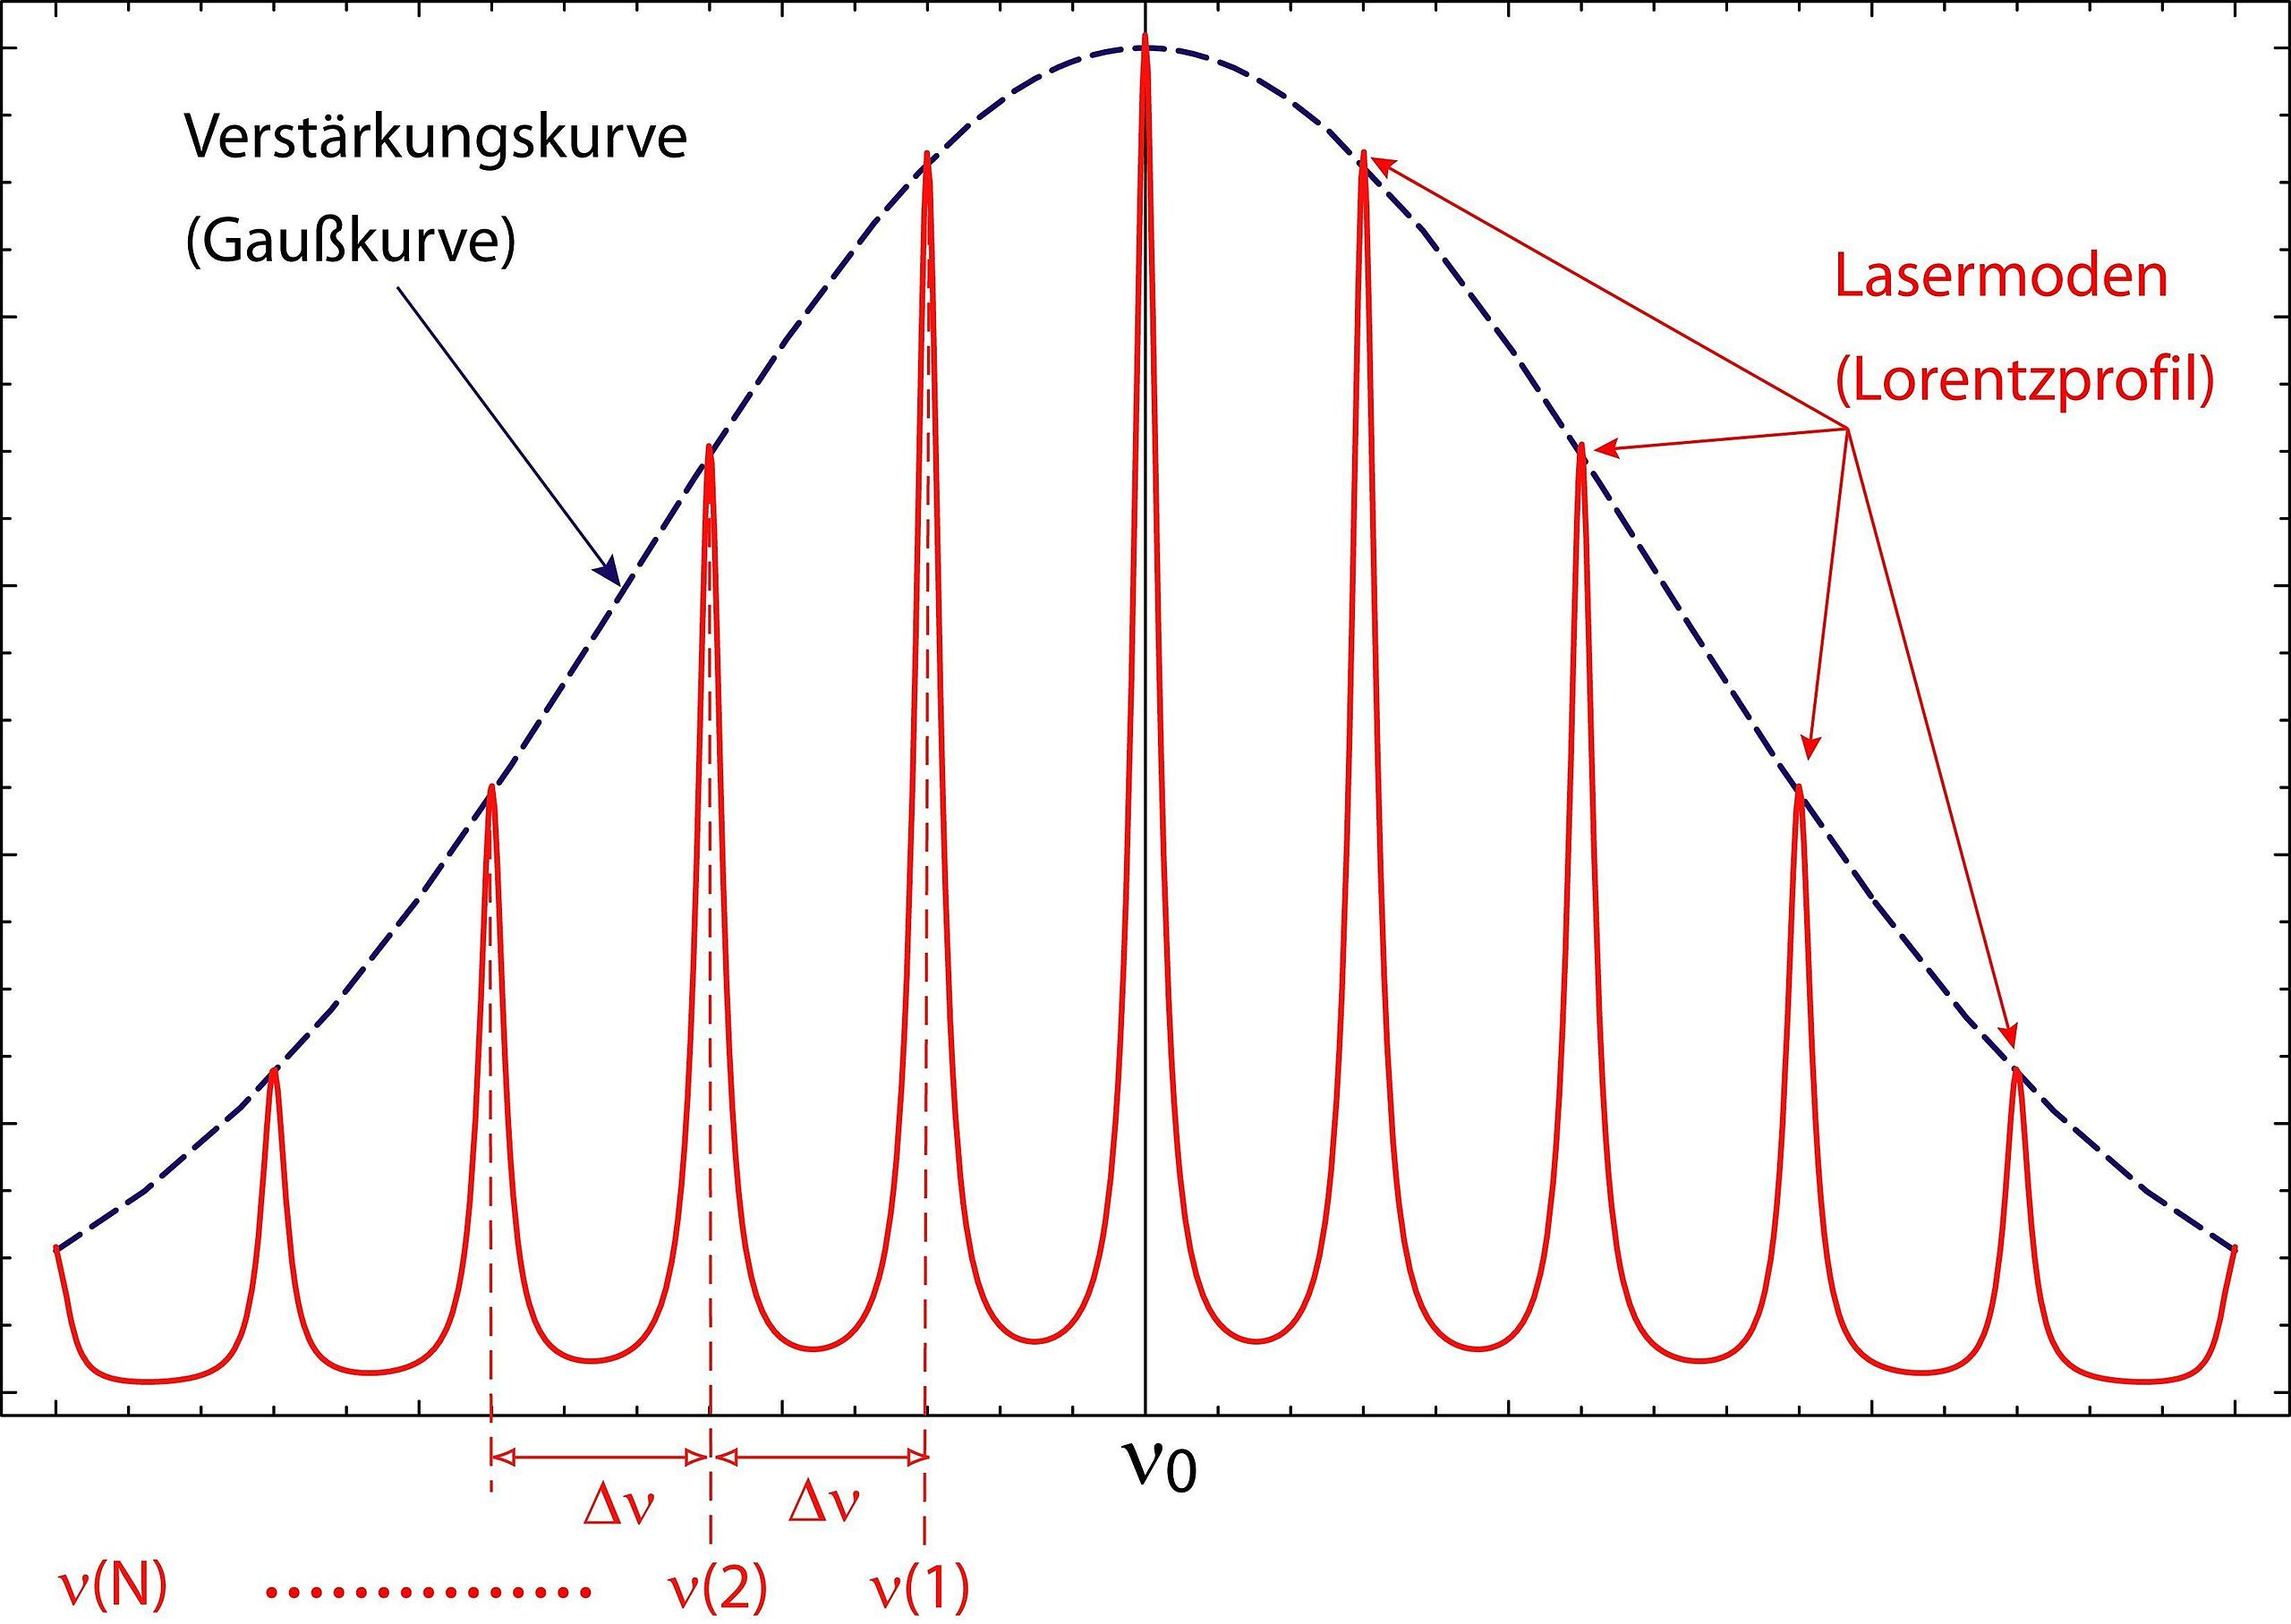
\includegraphics[width=0.6\textwidth]{FzV/LaserModes.jpg}
    \end{figure}
\end{center}
Die Bandbreite ist die Halbwertsbreite der Lasermoden.
Es werden nur solche angeregt, welche innerhalb der Verstärkungskurve (also dem Resonanzbereich) des Resonators liegen.\\\\
\textbf{single-mode Betrieb eines Lasers:}\\
Wenn man einen Laser mit einer hohen Wellenlängenstabilität benötigt, greift man oft auf einen single-mode Laser zurück.
Diese oszilliere nur auch einer Resonator-Eigenschwingung und geben somit nur eine Mode vonsich.
Praktisch wird dies so umgesetzt, das der Laserstrahl ein sogenanntes Fabry-Perot-Ethalon\footnote{Dünnes, beidseitig verspiegeltes Blättchen. Funktionsweise ähnlich zum Faby-Perot-Interferometer} passiert.
Eine Mode kann dies nur passieren und somit hat man eine sehr hohe Wellenlängenstabilität.
\section{Messung von Mischfrequenzen mittels einer Photodiode}
Im Resonator kann es vorkommen, dass die Frequenzen sich leicht unterscheiden.
Somit kommt es zu einer Mischfrequenz, einer Schwebung.
Diese Frequenzen kann man im Detektor nicht mehr detektieren, weswegen man aus der Schwebungsdifferenzfrequenz den Abstand der Moden bestimmt.
\section{Dielektrische Spiegel}
Der Dielektrische Spiegel, oder auch Bragg-Spiegel genannt, ist ein effizienter Reflektor und wird oft in optischen Resonatoren eingesetzt.
Diese besteht aus alternierenden, dünnen Schichten Dielektrika mit unterschiedlichen Brechungindizes.
An jeder dieser vielen Grenzschichten zwischen den einzelnen Lagen, wird ein Teil des Lichtes gemäß den Fesnelschen' Formeln reflektiert.
Ist die Wellenlänge des einfallenden Lichts ein Vielfaches der optischen Weglänge, so interferrieren die Wellen konstruktiv und es entsteht ein relativ guter Reflektor.
\section{3- und 4-Niveaulaser, Termschema für He-Ne-Laser}
\textbf{3- und 4-Niveaulaser}\\
Bei einem Drei-Niveaulaser sind 3 Energieniveaus an der Laseremission beteiligt.
Aus dem Grundzustand werden die Atome durch eine Pumpe in den hohen Zustand 2 (oberes Pumpenniveau) angeregt.
Von dort fällt es in das obere Laserniveau durch spontane Emission.
Um in den Grundzustand wieder zurückzukommen, nutzt man induzierte Emission.
Ein Beispiel für einen 3-Niveaulaser ist der Rubinlaser.
Ein Drei-Niveaulaser hat einen sehr schmale, aber intensive Laserlinie.\\
Bei einem Vier-Niveaulaser sind 4 Energieniveaus an der Laseremission beteiligt.
Hier ist der Unterschied, dass das Atom nicht wie beim Drei-Niveaulaser nach der induzierten Emission in das Grundniveau zurück fällt, sondern in einen weitern Zustand, den unteren Laserniveau.
Von dort fällt es durch spontane Emission in das Grundniveau zurück.
Ein Vorteil hierbei ist, dass die Besetzungsinversionen dauerhaft aufrechterhalten und die Pumpleistung verringer werden kann.
Damit ist ein Dauerstrichlaser realisierbar und nicht wie beim Drei-Niveaulaser ein Pulslaser.
\textbf{Termschema für He-Ne-Laser}\\
Das Termschema eine He-Ne-Lasers sieht wie folgt aus:
\begin{center}
    \begin{figure}[h]
        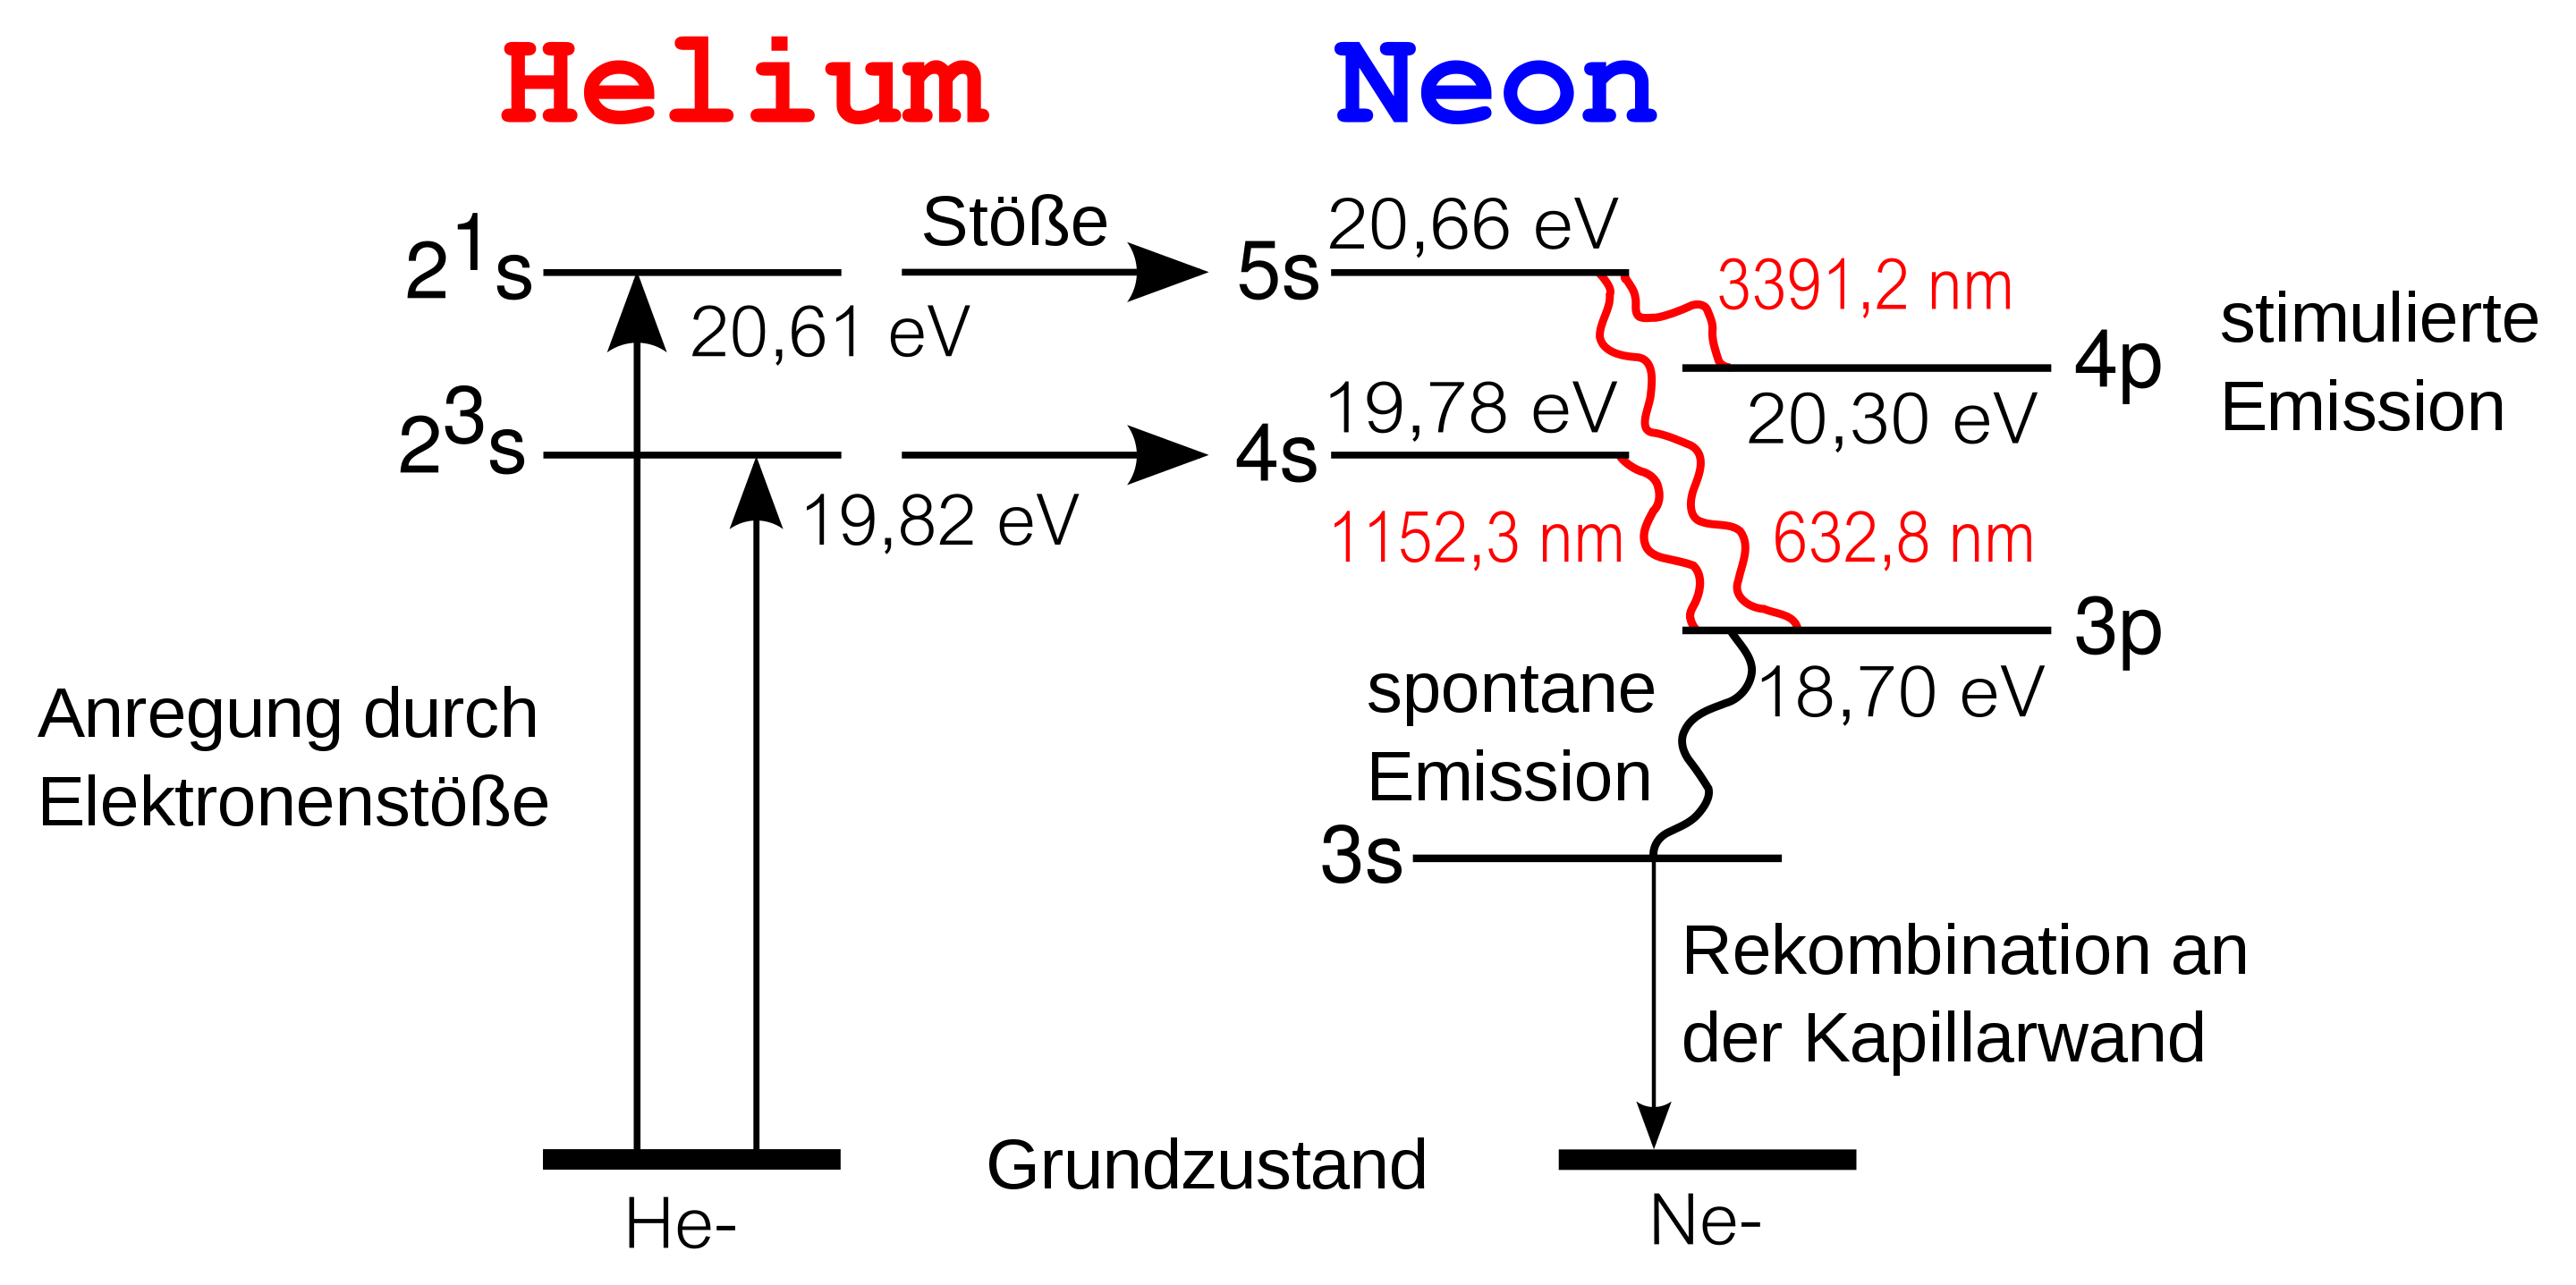
\includegraphics[width=0.6\textwidth]{FzV/TermschemaHeNe.png}
    \end{figure}
\end{center}

\section{Konfokales Fabry-Perot-Interferometer}
Das Fabry-Perot-Interferometer besteht aus zwei teilweise-durchlässigen Spiegel mit ein sehr hohen Reflexionsgrad.
Da durch Variieren des Abstands zwischen den beiden Spiegel sich der optische Weg verändert, kann es bei der Reflexion zu konstruktiver oder destruktiver Interferrenz kommen.
Dies sieht man dann an der Wand durch ein Ringmuster.
\section{Definition der Basiseinheit Meter}
Der Meter wurde definiert als diejenige Strecke, die das Licht im Vakuum innerhalb des Zeitintervalls von 1/299 792 458 Sekunden durchläuft.
\section{Gauß'sche Strahlen, Strahlausbreitung in Medien, Strahlausbreitungsfaktor M$^2$}
\textbf{Gauß'sche Strahlen}\\
Gauß'sche Strahlen sind ein Konzept der Wellenausbreitung in der paraxialen Optik.
Der Querschnitt des Strahles zeigt eine Gauskurve, mit einer in Ausbreitungsrichtung variierenden Breite.
\textbf{Strahlausbreitung in Medien}\\
Strahlen breiten sich in Medien so aus geradlinig aus, damit ihre Laufzeit extremal ist.
\textbf{Strahlausbreitungsfaktor M$^2$}\\
Die Strahlqualität eines Lasers wird durch den M2 Faktor charakteriesiert.
Dieser vergleicht die Form des Laserstrahles mit einem idealen Gauß-Strahls.
\section{Holographie}
Die Holographie beschreit die Aufnahme und Rekonstruktion eines Wellenfeldes, welches von einem beliebigen Objekt ausgeht.

